% Chapter Template

\chapter{Introduction} 
\label{chapter-introduction} 

%----------------------------------------------------------------------------------------
%	SECTION 
%----------------------------------------------------------------------------------------

\section{Motivation}

In recent years, there has been tremendous advances in the field of Artificial Intelligence (AI), especially in Deep Learning \citep{lecun-dl, deeplearning-overview}. Deep Learning has helped AI systems reach and sometimes surpass human-level perception, mostly in computer vision \citep{image-recognition} and natural language processing \citep{machine-translation}. Giving rise to amazing industrial application such as autonomous driving, early cancer detection, enhanced machine translation, etc. A primary concern of engineers is to make sure the trained models are error-free, which can be challenging if the input data does not carry enough information.

One possible solution researchers started to explore is to use multiple modalities\footnote{The term modality, also called mode, is generally understood to mean "the way in which something happened or is experienced" \citep{taxomany-multimodal}}, which makes sense since our experience of the world is multi-modal, i.e., we see objects, hear sound, feel the texture, smell odours, and taste flavours. Multi-Modal Deep Learning (MMDL) is used in the hope that the information carried by each mode is additive, such that the model can learn to make more accurate predictions. For example, in \citep{lidar-camera} sensorial inputs from wide angle cameras and LIDAR\footnote{Laser Detection and Ranging} sensors are combined for road detection. Cameras provide dense information over a long range under good illumination and fair weather, whereas LIDARs are only marginally affected by the external lighting conditions but have a limited range. Thus, merging the complementary information of the two sensors improves the road detection. Despite its efficacy, MMDL suffers from a major drawback: no explicit mechanisms exists to handle failing modes. In the present report, a mode is said to be failing if a) it contains a significant amount of noise, b) the data is much different from the training data, c) the data is missing. Failing modes a) and b) generally degrade the quality of the predictions because they introduce perturbations in the network.

On the other hand, humans seem to handle these situations robustly on a daily basis. A famous example showing this ability is called the cocktail-party effect \citep{cocktail-party}, it refers to the difficulty we sometimes have understanding speech in noisy social settings. As a subconscious response, we tend to look at the mouth of our interlocutor i.e. we shift some attention from the auditory to the visual senses. Similarly, our attention is shifted from vision to touch when we are wandering in a room where the lights suddenly switch off. These examples indicate that humans handle modes with perturbations (first example) or missing information (second example) by shifting their attention on the other more relevant modes \citep{crossmodal}.

Inspired from this behaviour, this report presents a new approach to tackle failing modes. I introduce a novel attention mechanism, named \textit{Energy-based Multi-Modal Attention} (EMMA), able to decide how much attention to devote to each mode, such that the relevant information is kept while masking out the perturbations. Additionally, this work offers some important insight into how current attention mechanisms in deep learning are surprisingly similar in some ways to attention in humans.

\begin{figure}[!ht]
\centering
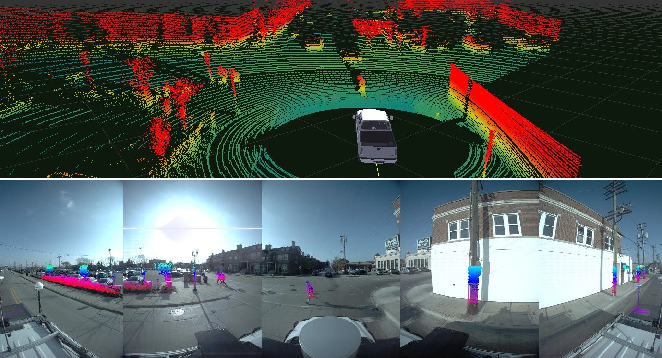
\includegraphics[scale=0.55]{figures/lidar-camera}
\caption[Lidar \& Camera view in self-driving cars]{Same environment, different modes (top: LIDAR view, bottom: camera view)}	
\label{fig:lidar-camera}
\end{figure}


%----------------------------------------------------------------------------------------
%	SECTION 
%----------------------------------------------------------------------------------------

\section{Proposed solution}\label{sec:proposed-solution}
The attention module EMMA is inserted in front of the model, focusing its attention on the modes such that the most useful information passes through while the perturbations are filtered out. The amount of attention distributed to a mode is based on its importance, encompassing three intrinsically tied properties:
\begin{itemize}
\item \textit{relevance}: the quantitative influence of the mode over the predictions
\item \textit{failure intensity}: a measure proportional to the outlyingness\footnote{The outlyingness of a data point tells us how far the observation lies from the center of the training set distribution} of the mode
\item \textit{coupling}: how does the information carried by the mode relate to the other modes? Is it redundant, complementary or conflicting?
\end{itemize}
Let us emphasize that determining the importance is sample dependent, and is thus not easily solved by learning the global tendency.
\begin{figure}[!h]
\centering
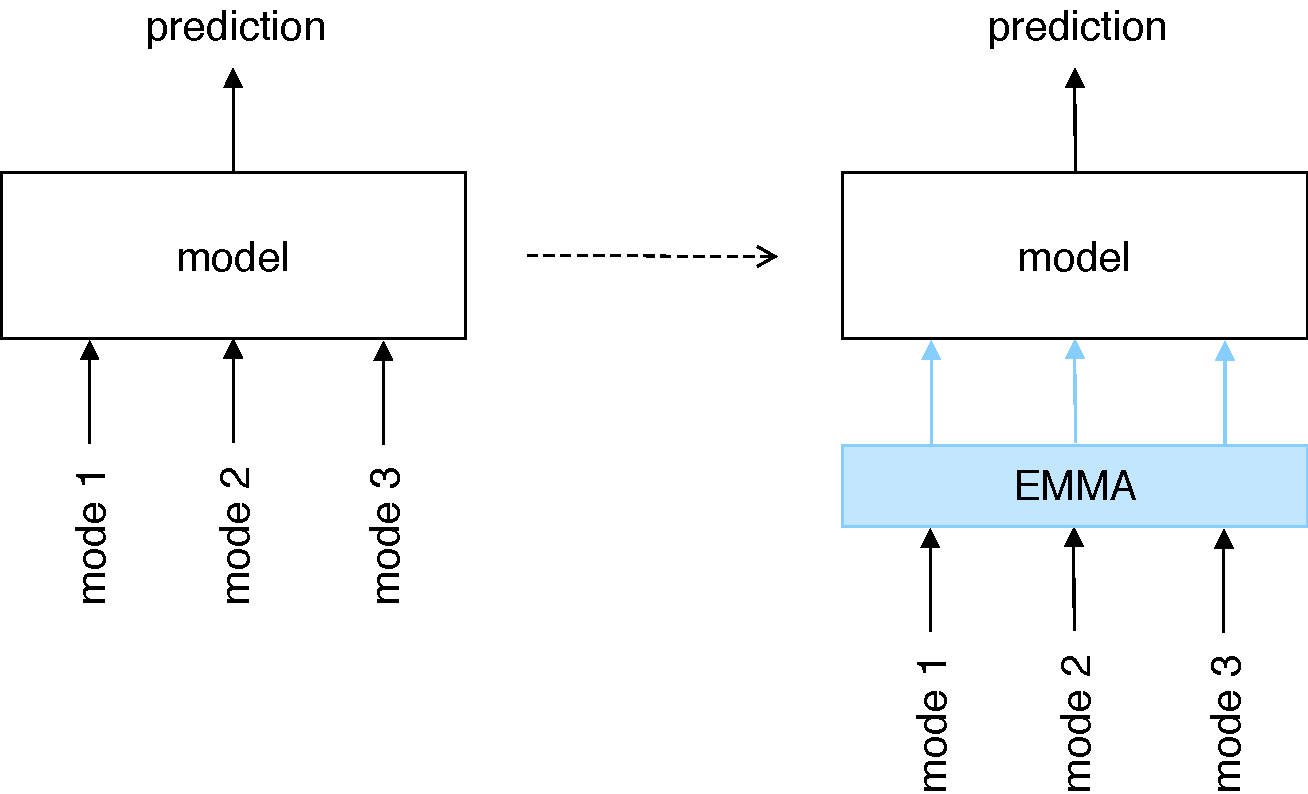
\includegraphics[scale=0.45]{figures/introduction-three-modes-with-emma}
\caption[Multi-Modal model with/without EMMA]{A multi-modal model with three input modes, without EMMA (left), improved with EMMA (right)}	
\label{fig:main-idea}
\end{figure}

\subsection*{Software Implementation}
All the implemented models and experiments are available at this \href{https://github.com/Werenne/energy-based-multimodal-attention}{repository}\footnote{\url{https://github.com/Werenne/energy-based-multimodal-attention}}, with a wiki explaining how to run the experiments; \href{https://pytorch.org/}{PyTorch}\footnote{\url{https://pytorch.org/}} was the main framework used regarding the Machine Learning part.

%----------------------------------------------------------------------------------------
%	SECTION 
%----------------------------------------------------------------------------------------

\section{Contributions}
The work presented in this Master thesis has led to three novel contributions.
\begin{description}
\item \textbf{Contribution 1: an attention module improving significantly the robustness against failing modes.} In Chapter \ref{chapter-emma}, we discuss the design of a new attention mechanism based on energy models \citep{ebm-tutorial}, that can be added to any multi-modal model. 
\item \textbf{Contribution 2: a simple yet powerful regularizer on attention mechanisms.} We slightly modify a common attention function permitting us to establish a link to the concept of capacity in psychology \citep{attention-is-effort}; Capacity is the amount of attention distributed among the inputs. Subsequently, a new regularizer is introduced to control the capacity, which we claim can help generalize against unexpected situations.
\item \textbf{Contribution 3: a unified model for multi-modal attention.} In Chapter \ref{chapter-literature-review}, a review of the literature on attention in humans helps us identify how to construct a more complete multi-modal attention module.
\end{description}

%----------------------------------------------------------------------------------------
%	SECTION 
%----------------------------------------------------------------------------------------

\section{Thesis Outline}
The remainder of this work is organised as follows.
\begin{description}
\item \textbf{Chapter 2} explains the background (i.e. deep learning and energy models) this work is based upon.
\item \textbf{Chapter 3} reviews the literature about attention in psychology and deep learning, and the similarities between them.
\item \textbf{Chapter 4} describes a method for the estimation of the failure intensity of a mode.
\item \textbf{Chapter 5} presents the ideas and architecture of the Energy-based Multi-Modal Attention module (Contribution 1 \& 2).
\item \textbf{Chapter 6} presents a thorough evaluation and analysis of the module outlined in Chapter \ref{chapter-emma}.
\item \textbf{Chapter 7} proposes a unified multi-modal attention module (Contribution 3).
\item \textbf{Chapter 8} concludes this work and suggests possible directions for future research.
\end{description}